\documentclass[CJK]{beamer}
\usepackage{CJKutf8}
\usepackage{beamerthemesplit}
\usetheme{Malmoe}
\useoutertheme[footline=authortitle]{miniframes}
\usepackage{amsmath}
\usepackage{amssymb}
\usepackage{graphicx}
\usepackage{eufrak}
\usepackage{color}
\usepackage{slashed}
\usepackage{simplewick}
\usepackage{tikz}
\usepackage{tcolorbox}
\graphicspath{{../figures/}}
%%figures
\def\lfig#1#2{\includegraphics[width=#1 in]{#2}}
\def\addfig#1#2{\begin{center}\includegraphics[width=#1 in]{#2}\end{center}}
\def\wulian{
\includegraphics[width=0.18in]{emoji_wulian.jpg}}
\def\bigwulian{
\includegraphics[width=0.35in]{emoji_wulian.jpg}}
\def\bye{
\includegraphics[width=0.18in]{emoji_bye.jpg}}
\def\bigbye{
\includegraphics[width=0.35in]{emoji_bye.jpg}}
\def\huaixiao{
\includegraphics[width=0.18in]{emoji_huaixiao.jpg}}
\def\bighuaixiao{
\includegraphics[width=0.35in]{emoji_huaixiao.jpg}}
%% colors
\def\blacktext#1{{\color{black}#1}}
\def\bluetext#1{{\color{blue}#1}}
\def\redtext#1{{\color{red}#1}}
\def\darkbluetext#1{{\color[rgb]{0,0.2,0.6}#1}}
\def\skybluetext#1{{\color[rgb]{0.2,0.7,1.}#1}}
\def\cyantext#1{{\color[rgb]{0.,0.5,0.5}#1}}
\def\greentext#1{{\color[rgb]{0,0.7,0.1}#1}}
\def\darkgray{\color[rgb]{0.2,0.2,0.2}}
\def\lightgray{\color[rgb]{0.6,0.6,0.6}}
\def\gray{\color[rgb]{0.4,0.4,0.4}}
\def\blue{\color{blue}}
\def\red{\color{red}}
\def\green{\color{green}}
\def\darkgreen{\color[rgb]{0,0.4,0.1}}
\def\darkblue{\color[rgb]{0,0.2,0.6}}
\def\skyblue{\color[rgb]{0.2,0.7,1.}}
%%control
\def\be{\begin{equation}}
\def\ee{\nonumber\end{equation}}
\def\bea{\begin{eqnarray}}
\def\eea{\nonumber\end{eqnarray}}
\def\bch{\begin{CJK}{UTF8}{gbsn}}
\def\ech{\end{CJK}}
\def\bitem{\begin{itemize}}
\def\eitem{\end{itemize}}
\def\bcenter{\begin{center}}
\def\ecenter{\end{center}}
\def\bex{\begin{minipage}{0.2\textwidth}
\includegraphics[width=0.6in]{jugelizi.png}\end{minipage}\begin{minipage}{0.76\textwidth}}
\def\eex{\end{minipage}}
\def\chtitle#1{\frametitle{\bch#1\ech}}
\def\bmat#1{\left(\begin{array}{#1}}
\def\emat{\end{array}\right)}
\def\bcase#1{\left\{\begin{array}{#1}}
\def\ecase{\end{array}\right.}
\def\bmini#1{\begin{minipage}{#1\textwidth}}
\def\emini{\end{minipage}}
\def\tbox#1{\begin{tcolorbox}#1\end{tcolorbox}}
\def\pfrac#1#2#3{\left(\frac{\partial #1}{\partial #2}\right)_{#3}}
%%symbols
\def\sone{$\star$}
\def\stwo{$\star\star$}
\def\sthree{$\star\star\star$}
\def\sfour{$\star\star\star\star$}
\def\sfive{$\star\star\star\star\star$}
\def\rint{{\int_\leftrightarrow}}
\def\roint{{\oint_\leftrightarrow}}
\def\stdHf{{\textit{\r H}_f}}
\def\deltaH{{\Delta \textit{\r H}}}
\def\ii{{\dot{\imath}}}
\def\skipline{{\vskip0.1in}}
\def\skiplines{{\vskip0.2in}}
\def\lagr{{\mathcal{L}}}
\def\hamil{{\mathcal{H}}}
\def\vecv{{\mathbf{v}}}
\def\vecx{{\mathbf{x}}}
\def\vecy{{\mathbf{y}}}
\def\veck{{\mathbf{k}}}
\def\vecp{{\mathbf{p}}}
\def\vecn{{\mathbf{n}}}
\def\vecA{{\mathbf{A}}}
\def\vecP{{\mathbf{P}}}
\def\vecsigma{{\mathbf{\sigma}}}
\def\hatJn{{\hat{J_\vecn}}}
\def\hatJx{{\hat{J_x}}}
\def\hatJy{{\hat{J_y}}}
\def\hatJz{{\hat{J_z}}}
\def\hatj#1{\hat{J_{#1}}}
\def\hatphi{{\hat{\phi}}}
\def\hatq{{\hat{q}}}
\def\hatpi{{\hat{\pi}}}
\def\vel{\upsilon}
\def\Dint{{\mathcal{D}}}
\def\adag{{\hat{a}^\dagger}}
\def\bdag{{\hat{b}^\dagger}}
\def\cdag{{\hat{c}^\dagger}}
\def\ddag{{\hat{d}^\dagger}}
\def\hata{{\hat{a}}}
\def\hatb{{\hat{b}}}
\def\hatc{{\hat{c}}}
\def\hatd{{\hat{d}}}
\def\hatN{{\hat{N}}}
\def\hatH{{\hat{H}}}
\def\hatp{{\hat{p}}}
\def\Fup{{F^{\mu\nu}}}
\def\Fdown{{F_{\mu\nu}}}
\def\newl{\nonumber \\}
\def\vece{\mathrm{e}}
\def\calM{{\mathcal{M}}}
\def\calT{{\mathcal{T}}}
\def\calR{{\mathcal{R}}}
\def\barpsi{\bar{\psi}}
\def\baru{\bar{u}}
\def\barv{\bar{\upsilon}}
\def\qeq{\stackrel{?}{=}}
\def\torder#1{\mathcal{T}\left(#1\right)}
\def\rorder#1{\mathcal{R}\left(#1\right)}
\def\contr#1#2{\contraction{}{#1}{}{#2}#1#2}
\def\trof#1{\mathrm{Tr}\left(#1\right)}
\def\trace{\mathrm{Tr}}
\def\comm#1{\ \ \ \left(\mathrm{used}\ #1\right)}
\def\tcomm#1{\ \ \ (\text{#1})}
\def\slp{\slashed{p}}
\def\slk{\slashed{k}}
\def\calp{{\mathfrak{p}}}
\def\veccalp{\mathbf{\mathfrak{p}}}
\def\Tthree{T_{\tiny \textcircled{3}}}
\def\pthree{p_{\tiny \textcircled{3}}}
\def\dbar{{\,\mathchar'26\mkern-12mu d}}
\def\erf{\mathrm{erf}}
\def\const{\mathrm{constant}}
\def\pheat{\pfrac p{\ln T}V}
\def\vheat{\pfrac V{\ln T}p}
%%units
\def\fdeg{{^\circ \mathrm{F}}}
\def\cdeg{^\circ \mathrm{C}}
\def\atm{\,\mathrm{atm}}
\def\angstrom{\,\text{\AA}}
\def\SIL{\,\mathrm{L}}
\def\SIkm{\,\mathrm{km}}
\def\SIyr{\,\mathrm{yr}}
\def\SIGyr{\,\mathrm{Gyr}}
\def\SIV{\,\mathrm{V}}
\def\SImV{\,\mathrm{mV}}
\def\SIeV{\,\mathrm{eV}}
\def\SIkeV{\,\mathrm{keV}}
\def\SIMeV{\,\mathrm{MeV}}
\def\SIGeV{\,\mathrm{GeV}}
\def\SIcal{\,\mathrm{cal}}
\def\SIkcal{\,\mathrm{kcal}}
\def\SImol{\,\mathrm{mol}}
\def\SIN{\,\mathrm{N}}
\def\SIHz{\,\mathrm{Hz}}
\def\SIm{\,\mathrm{m}}
\def\SIcm{\,\mathrm{cm}}
\def\SIfm{\,\mathrm{fm}}
\def\SImm{\,\mathrm{mm}}
\def\SInm{\,\mathrm{nm}}
\def\SImum{\,\mathrm{\mu m}}
\def\SIJ{\,\mathrm{J}}
\def\SIW{\,\mathrm{W}}
\def\SIkJ{\,\mathrm{kJ}}
\def\SIs{\,\mathrm{s}}
\def\SIkg{\,\mathrm{kg}}
\def\SIg{\,\mathrm{g}}
\def\SIK{\,\mathrm{K}}
\def\SImmHg{\,\mathrm{mmHg}}
\def\SIPa{\,\mathrm{Pa}}

\title{Lesson 01 - 1st Law of Thermal Dynamics}
  \author{}
  \date{}


\begin{document}

\begin{frame}
\begin{center}
\begin{Large}
\bch
热学 \\
第1讲 温度,温标和理想气体

{\vskip 0.3in}

黄志琦

\ech
\end{Large}
\end{center}

\vskip 0.2in

\bch
教材:《热学》第二版,赵凯华,罗蔚茵,高等教育出版社
\ech

\bch
课件下载
\ech
https://github.com/zqhuang/SYSU\_TD
\end{frame}


\begin{frame}
\chtitle{温度(Temperature): 热的强度}
\bch
{\large 

\skiplines

\bmini{0.5}
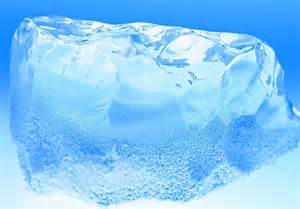
\includegraphics[width = 2in]{ice.jpeg}

温度低
\emini
\bmini{0.4}
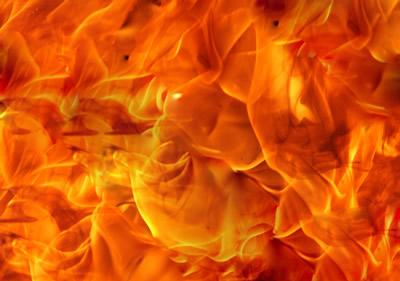
\includegraphics[width = 2in]{fire.jpg}

温度高
\emini
}
\ech
\end{frame}


\begin{frame}
\chtitle{温标(Temperature Scale): 温度的数值表示法}
\bch

日常用温标:
\skiplines

\bmini{0.35}
华氏温标($\fdeg$)

(Fahrenheit scale)
\emini
\bmini{0.25}
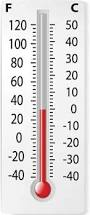
\includegraphics[width=0.6in]{thermometer.jpg}
\emini
\bmini{0.35}
摄氏温标($\cdeg$)

(Celsius scale)
\emini

\ech
\end{frame}


\begin{frame}
\chtitle{摄氏度和华氏度之间的转换}
\bch
\skipline
转换口诀:{\bf 三十二冰,九华五摄。}
\begin{itemize}
\item{$32\fdeg$和$0\cdeg$度等价,是(1 atm下)水的冰点;}
\item{超过或者不足冰点部分,按照$9\fdeg$等价于$5\cdeg$换算。}
\end{itemize}

\skiplines

请举手抢答:一个标准大气压下水的沸点是多少华氏度?
\ech
\end{frame}



\begin{frame}
\chtitle{温标的定义方法}
\bch
以水银温度计校准的摄(华)氏温标为例:
\bmini{0.8}
\begin{itemize}
\item{{\bf 固定标准点}:规定一个标准大气压下,水的冰点为$0\cdeg$ ($32\fdeg$),水的沸点为$100\cdeg$ ($212\fdeg$)。}
\item{{\bf 测温物质}: 水银。}
\item{{\bf 测温属性}: 热胀冷缩,规定温度与水银体积成线性关系。} 
\end{itemize}
\emini
\bmini{0.15}
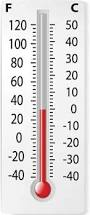
\includegraphics[width=0.6in]{thermometer.jpg}
\emini

\skipline

一般地,定义一个温标需要上述三要素:固定标准点,测温物质,测温属性。
\ech
\end{frame}

\begin{frame}
\chtitle{幻想实验:标度一个水银温度计}
\bch
\bmini{0.3}
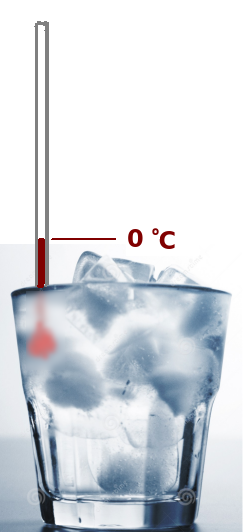
\includegraphics[width=0.8in]{scale0deg.png}

{\scriptsize 1)放入1 atm下的冰水混合物,达到热平衡时在水银柱最高处标上$0\cdeg$。}
\emini
\hspace{0.1in}
\bmini{0.3}
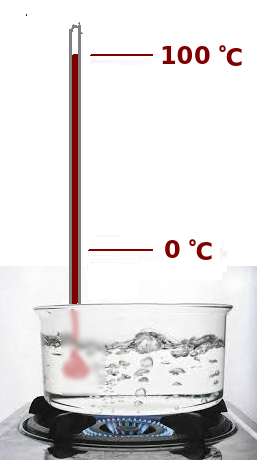
\includegraphics[width=0.8in]{scale100deg.png}

{\vskip 0.3in}

{\scriptsize 2)放入1 atm下的沸水,达到热平衡时在水银柱最高处标上$100\cdeg$。}
\emini
\hspace{0.1in}
\bmini{0.3}
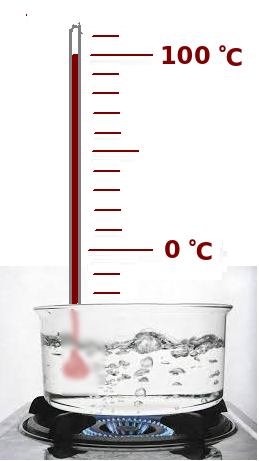
\includegraphics[width=0.8in]{scalefull.png}

{\vskip 0.3in}

{\scriptsize 3)均匀地标上其他刻度

\vspace{0.36in} 

}
\emini
\ech
\end{frame}

\begin{frame}
\bch
刚刚复习了一些小学知识,下面我们要进行深邃的思考……

\begin{center}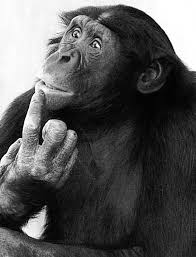
\includegraphics[width=1in]{think.jpg}\end{center}
\ech
\end{frame}


\begin{frame}
\bch
\bmini{0.2}
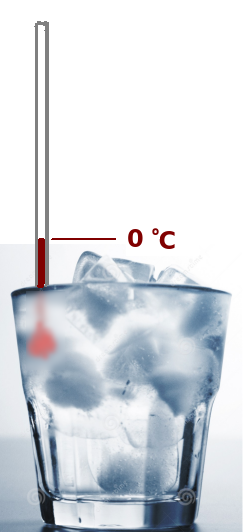
\includegraphics[width=0.8in]{scale0deg.png}
\emini
\bmini{0.75}
\begin{itemize}
\item[1]{ “热平衡”是什么?}
\item[2]{ 为什么我们认为(或者说,能够规定)达到热平衡时的温度计与冰水混合物的温度相同?}
\end{itemize}
\emini
\ech
\end{frame}


\begin{frame}
\chtitle{热平衡}
\bch
在外界条件影响隔绝的条件下,当两个宏观物体发生接触时,可能发生热传导,力的相互作用,化学反应,电磁相互作用等。

\skipline

物体所有宏观性质不发生变化 = 热平衡 + 力学平衡 + 化学平衡 + 电磁平衡 + ... 

\skiplines

在我们的幻想实验里,我们用真空玻璃管隔离了水银和冰水混合物,使得它们之间只能发生热传导,在这个设定下:

\skipline

物体所有宏观性质不发生变化 = 热平衡

\ech
\end{frame}

\begin{frame}
\chtitle{热力学第零定律}
\bch
{\large \bluetext{在外界影响隔绝的条件下,如果物体A、B分别与{\bf 处于确定状态}的物体C达到热平衡,则物体A和B也是相互热平衡的。}}

\skiplines

comments:
\begin{itemize}
\item{“在外界影响隔绝的条件下”是一句很正确的废话。{\small(既然讨论热平衡,就已经假定了这个条件。)}}
\item{要求C“处于确定状态”非常重要。(如果去掉“处于确定状态”,请试举个反例)}
\item{热力学第零定律是一条实验定律。}
\item{有了热力学第零定律,我们就能规定所有达到热平衡的物体具有相同的温度。}
\end{itemize}
\ech
\end{frame}

\begin{frame}
\bch
解决了水银温度计的标度问题,我们再进一步思考更深邃的问题……
\begin{center}
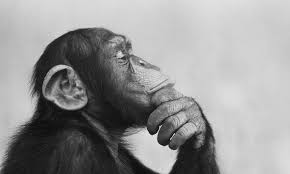
\includegraphics[width=2in]{think2.jpg}
\end{center}
\ech
\end{frame}

\begin{frame}
\chtitle{更深邃的问题1}
\bch
一定要用水银作为测温物质吗?

\skiplines

\begin{itemize}
\item{如果用酒精,固定压强的气体等代替水银,因为我们人为地“规定”了温度随体积线性地变化,那么水银温标和酒精温标、气体温标并不一定会完全相同。}
\item{日常所需测量的温度往往不需要非常精确,不同温标之间的微小差异(一般不大于$0.1\cdeg$的数量级)可以忽略。}
\end{itemize}

\ech
\end{frame}


\begin{frame}
\chtitle{更深邃的问题2}
\bch
一定要用热胀冷缩的测温属性吗?

\skipline

\bitem
\item{除了热胀冷缩,温变电阻金属的电阻随温度变化,热电偶效应等也都可以用来定义温标。}
\item{不同测温属性定义的温标不完全相同,但日常测温需求往往可以忽略这些差别。}
\eitem

\bcenter
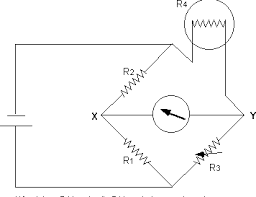
\includegraphics[width=1.4in]{resistance_thermometer.png}\hspace{0.1in}
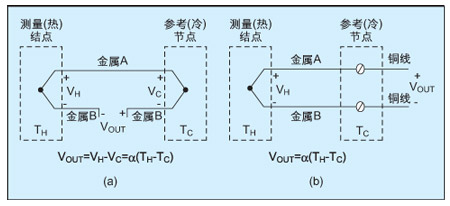
\includegraphics[width=2.2in]{thermocouple2.jpg}
\ecenter
\ech
\end{frame}


\begin{frame}
\chtitle{更深邃的问题3}
\bch
除了水的冰点和沸点,还有其他固定标准点吗?

\skipline

\bitem
\item{有。例如{\bf 绝对零度}和{\bf 水的三相点}都是更好的固定标准点。(\wulian 这些都是什么鬼)}
\eitem

\ech
\end{frame}

\begin{frame}
\chtitle{感想}
\bch
学习了这么多温标,真是太开心了\wulian

\skiplines

大学套路深,我要回小学\wulian

\skiplines

能不能就爽快点告诉我,以后我们用哪种温标\wulian

\ech
\end{frame}


\begin{frame}
\chtitle{告诉你们一个好消息}
\bch
前面讲的温标,以后我们都不用\bye
\ech
\end{frame}

\begin{frame}
\chtitle{热力学温标}
\bch
在热力学里我们使用热力学温标。

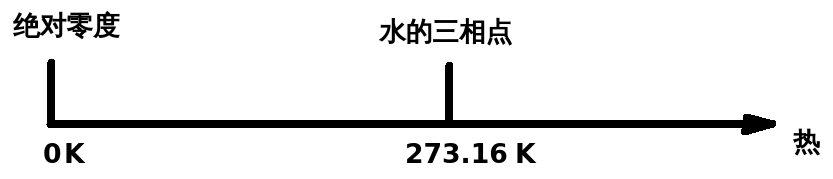
\includegraphics[width=3in]{absoluteTdef.png}
\bitem
\item{热力学温标的定义不涉及测温物质和测温属性。{\small \darkgray(所谓的“三要素”是逗你玩的\bye)}}
\item{热力学温标选取的固定标准点为绝对零度(规定为$0K$)和水的三相点(规定为$273.16K$)。 {\small \darkgray(是不是除了数字什么也没看懂\bye)}}
\eitem

{\small
取$273.16K$这个特定的数字是为了使$1K$的温度变化和$1\cdeg$的温度变化非常接近。}
\ech
\end{frame}


\begin{frame}
\chtitle{热力学温标和摄氏温标之间的转换}
\bch
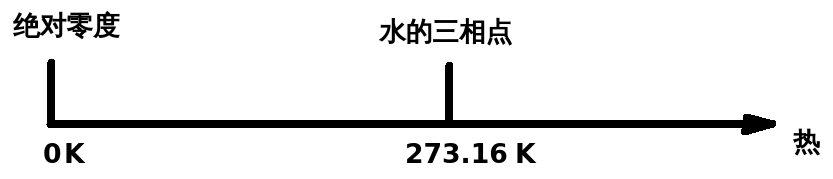
\includegraphics[width=3in]{absoluteTdef.png}

一般不指定特定的测温物质时,我们就认为变化$1\cdeg$等价于变化$1K$。 

在摄氏温标中,水的三相点为$0.01\cdeg$,对应于热力学温度$273.16K$。所以摄氏温标转换到热力学温标只需数值上平移$273.15$。例如: 
$$0\cdeg = 273.15 K$$
$$100\cdeg = 373.15K$$
$$0K = -273.15 \cdeg$$
\ech
\end{frame}

\begin{frame}
\chtitle{等等,还有很多疑问}
\bch
\bitem
\item{热力学温标是如何做到不依赖测温物质和测温属性进行标度的?}
\item{什么是绝对零度?为什么没有比绝对零度更低的温度?}
\item{什么是水的三相点?为什么它不像冰点和沸点那样依赖于压强?}
\eitem
\ech
\end{frame}


\begin{frame}
\chtitle{热力学温度也可以等价地用理想气体来标度}
\bch
热力学温标的诸多问题都比较深刻,将在后面的课程中逐步介绍。

\skiplines

我们先介绍一个用理想气体标度热力学温度的简单方法(即和热力学温标等价的理想气体温标)。

\skiplines


理想气体是把稀薄的实际气体进行理想化的一种假想物质。从微观上描述,理想气体分子有如下特性:
\bitem
\item{分子的大小远远小于分子之间平均距离。}
\item{除了分子之间以及分子和容器壁之间发生时间短暂得可以忽略的弹性碰撞外,分子不受任何外力作用做匀速直线运动。}
\eitem
常温下的实际稀薄的气体的属性非常接近理想气体。

\ech
\end{frame}



\begin{frame}
\chtitle{用理想气体标度热力学温度的理论根据——理想气体状态方程}
\bch
{\large 达到平衡状态的理想气体的摩尔数$\nu$, 压强$p$, 体积$V$,热力学温度$T$满足
{\color{blue}
$$p V = \nu RT$$
}
其中$R=8.31 \mathrm{J/(mol\cdot K)}$为{\bf 普适气体常量}。
}

{\small
\begin{itemize}
\item{回顾下“摩尔”的定义:每mol 物质包含 $6.02\times 10^{23}$个微粒。}
\item{固定$p$, $V$, $T$中的一个即分别得到历史上的气体实验定律:盖吕萨克定律,查理定律,波意耳定律。}
\item{从理想气体状态方程可以推出化学课上学过的阿伏伽德罗定律:标准状态($1$ atm, $0\cdeg$)下1 mol理想气体的体积为$22.4L$。}
\end{itemize}
}
\ech
\end{frame}

\begin{frame}
\chtitle{用理想气体标度热力学温度:气体温度计}
\bch

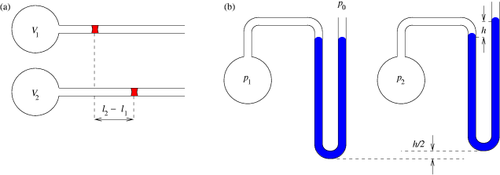
\includegraphics[width=3.2in]{gas_thermometer.png}


定压气体温度计 \hspace{0.5in} 定体气体温度计

固定$p$,$T\propto V$ \hspace{0.6in}  固定$V$,$T\propto p$

\ech
\end{frame}


\begin{frame}
\bch
下面我们讲关于热力学温度的一些补充知识
\ech
\end{frame}

\begin{frame}
\chtitle{热力学温度的微观意义}
\bch
\bitem
\item{物质是由微观粒子(分子或者原子)组成的。温度越高,代表微观粒子的能量越高(对于气体分子而言,这就意味着粒子的运动越剧烈)。}
\item{统计上讲,微观粒子总是更趋向于能量低的状态。一个微观状态的能量越高,粒子处在这个状态上的概率越小。粒子在各个微观状态上的出现概率,随各个状态的能量呈现一个指数衰减的规律,且衰减率反比于热力学温度。

具体地讲,假设粒子可以处在状态$1,2,3,\ldots$每个状态的能量分别为$\varepsilon_1$, $\varepsilon_2$, $\varepsilon_3$, $\ldots$那么粒子处在某状态$i$的概率正比于
$$e^{-\frac{\epsilon_i}{k T}}\, ,$$其中$k=1.38\times 10^{-23} J/K$为玻尔兹曼常数。
}
\eitem

\ech
\end{frame}

\begin{frame}
\chtitle{理想气体分子的位置和速度分布}
\bch
理想气体分子的状态由位置$\mathbf{x} = (x_1, x_2, x_3)$和速度$\mathbf{\upsilon} = (\upsilon_1, \upsilon_2, \upsilon_3)$来描述。也就是说,分子的每一个状态对应于位置空间的一个点$(x_1, x_2, x_3)$和"速度空间"({\darkblue 这是我们假想的一个空间,和“看得见摸得着”的位置空间不同})的一个点$(\upsilon_1, \upsilon_2, \upsilon_3)$。

\skipline

由于位置和能量无关,分子处在容器内任何位置的概率相同。

\skipline

由于速度和能量的关系为$\varepsilon = \frac{1}{2} m \upsilon^2$,其中$m$为分子质量,所以分子处在速度为$\mathbf{\upsilon}$的状态的概率正比于
$$e^{-\frac{m\upsilon^2}{2kT}}$$


\ech
\end{frame}

\begin{frame}
\chtitle{理想气体分子的位置和速度分布(续)}
\bch

在速度空间中,考虑半径在$\upsilon$和$\upsilon+d\upsilon$之间的一层“球壳”。速度点落在这个球壳内的微观状态的数目正比于球壳的体积$4\pi \upsilon^2 d\upsilon$(这里我们假定了速度空间是离散化的,且每个微观状态占据的体积相等)。

综上,分子速率在$\upsilon$和$\upsilon+d\upsilon$的概率正比于微观态数目和落在微观态上的概率的乘积,即

$$(4\pi \upsilon^2 d\upsilon) (e^{-\frac{m\upsilon^2}{2kT}}) \propto  \upsilon^2 e^{-\frac{m\upsilon^2}{2kT}} d\upsilon  $$


\ech
\end{frame}

\begin{frame}
\chtitle{理想气体分子的平均动能}
\bch
理想气体分子的平均动能只需要对各个速率的分子的动能按出现概率进行加权平均:

{\scriptsize
\bea
\bar\varepsilon &=& \frac{\int_0^\infty (\frac{1}{2}m\upsilon^2) \upsilon^2 e^{-\frac{m\upsilon^2}{2kT}} d\upsilon}{\int_0^\infty \upsilon^2 e^{-\frac{m\upsilon^2}{2kT}} d\upsilon} \newl
&=& \frac{-\frac{kT}{2}\int_0^\infty  \upsilon^3 d\left(e^{-\frac{m\upsilon^2}{2kT}}\right) }{\int_0^\infty \upsilon^2 e^{-\frac{m\upsilon^2}{2kT}} d\upsilon} \newl
&=& \frac{-\frac{kT}{2}\left[ \left.\upsilon^3 e^{-\frac{m\upsilon^2}{2kT}}\right\vert^{\infty}_{0} - \int_0^\infty e^{-\frac{m\upsilon^2}{2kT}} d\left(\upsilon^3\right)\right]}{\int_0^\infty \upsilon^2 e^{-\frac{m\upsilon^2}{2kT}} d\upsilon} \newl
&=&\frac{\frac{3kT}{2} \int_0^\infty \upsilon^2 e^{-\frac{m\upsilon^2}{2kT}} d \upsilon}{\int_0^\infty \upsilon^2 e^{-\frac{m\upsilon^2}{2kT}} d\upsilon} \newl
&=&\frac{3kT}{2}
\eea
}
\ech
\end{frame}




\end{document}
